%%
%% This is file `sample-authordraft.tex',
%% generated with the docstrip utility.
%%
%% The original source files were:
%%
%% samples.dtx  (with options: `authordraft')
%% 
%% IMPORTANT NOTICE:
%% 
%% For the copyright see the source file.
%% 
%% Any modified versions of this file must be renamed
%% with new filenames distinct from sample-authordraft.tex.
%% 
%% For distribution of the original source see the terms
%% for copying and modification in the file samples.dtx.
%% 
%% This generated file may be distributed as long as the
%% original source files, as listed above, are part of the
%% same distribution. (The sources need not necessarily be
%% in the same archive or directory.)
%%
%% The first command in your LaTeX source must be the \documentclass command.
\documentclass[sigconf,  review=false, nonacm=true]{acmart}
%% NOTE that a single column version may required for 
%% submission and peer review. This can be done by changing
%% the \doucmentclass[...]{acmart} in this template to 
%% \documentclass[manuscript,screen]{acmart}
%% 
%% To ensure 100% compatibility, please check the white list of
%% approved LaTeX packages to be used with the Master Article Template at
%% https://www.acm.org/publications/taps/whitelist-of-latex-packages 
%% before creating your document. The white list page provides 
%% information on how to submit additional LaTeX packages for 
%% review and adoption.
%% Fonts used in the template cannot be substituted; margin 
%% adjustments are not allowed.

%%
%% \BibTeX command to typeset BibTeX logo in the docs
\AtBeginDocument{%
  \providecommand\BibTeX{{%
    \normalfont B\kern-0.5em{\scshape i\kern-0.25em b}\kern-0.8em\TeX}}}



%%
%% Submission ID.
%% Use this when submitting an article to a sponsored event. You'll
%% receive a unique submission ID from the organizers
%% of the event, and this ID should be used as the parameter to this command.
%%\acmSubmissionID{123-A56-BU3}

%%
%% The majority of ACM publications use numbered citations and
%% references.  The command \citestyle{authoryear} switches to the
%% "author year" style.
%%
%% If you are preparing content for an event
%% sponsored by ACM SIGGRAPH, you must use the "author year" style of
%% citations and references.
%% Uncommenting
%% the next command will enable that style.
%%\citestyle{acmauthoryear}

\setcitestyle{sort}

%%
%% end of the preamble, start of the body of the document source.
\usepackage{multirow}
\usepackage{graphicx}
\usepackage{float}

\begin{document}

%%
%% The "title" command has an optional parameter,
%% allowing the author to define a "short title" to be used in page headers.
\title{Detecting Sarcasm and Irony in Texts: An Overview}

%%
%% The "author" command and its associated commands are used to define
%% the authors and their affiliations.
%% Of note is the shared affiliation of the first two authors, and the
%% "authornote" and "authornotemark" commands
%% used to denote shared contribution to the research.
\author{Denis Reibel}
\email{denis.reibel@uni-ulm.de}
\affiliation{%
  \institution{Institute of Databases and Information Systems}
  \city{University Ulm}
  \country{Germany}
}

%%
%% By default, the full list of authors will be used in the page
%% headers. Often, this list is too long, and will overlap
%% other information printed in the page headers. This command allows
%% the author to define a more concise list
%% of authors' names for this purpose.
\renewcommand{\shortauthors}{Denis Reibel}

%%
%% The abstract is a short summary of the work to be presented in the
%% article.
\begin{abstract}
  The field of sarcasm and irony detection in texts holds some difficult problems that haven't been solved yet. However a lot of research was done lately. In this work we provide an overlook over the current state of the research field. It's most challenging problems are explain why it's especially challenging. We clustered attempts to classify sarcasm made by other researchers into six different method groups. The groups are compared and some techniques used in sarcasm classification are discussed, regarding their advantages and disadvantages.
\end{abstract}

%%
%% Keywords. The author(s) should pick words that accurately describe
%% the work being presented. Separate the keywords with commas.
\keywords{natural language processing, sentiment analysis, sarcasm detection}

\begin{teaserfigure}
  \centering
  
\includegraphics[width=0.5\textwidth]{./sources/teaser_tweet}
  \caption{American comedian Stephen Colbert tweeting about climate change}
  \Description{American comedian Stephen Colbert makes a sarcastic tweet about climate change}
  \label{fig:teaser}
\end{teaserfigure}

% enabling page numbers
\settopmatter{printacmref=false, printccs=true, printfolios=true}

%%
%% This command processes the author and affiliation and title
%% information and builds the first part of the formatted document.
\maketitle

%% Feedback
%% Nice presentation in English; well organized presentation
%% * Good to have a Section 2 on Language Theory
%% * Good organization of the methods in Section (grouping); Please 
%% capitalize the first letter of subsections, e.g. "4.4 learning " --> 
%% "4.4 Learning"
%% * Good choice of adding the eyetracking work! -> very interesting.
%% * Detailed analysis (discussion) and reflection
%% * English is very good,
%% Chapter Two -> Section 2 (egal auch welche Unterstruktur, im Paper ist 
%% es immer Section X.Y)
%% Don't capitalize "Problems in Sarcasm Detection"
%% "I grouped similar" -> "We grouped..." or "The methods are grouped 
%% into..." (also use plural/passive voice)
%% When something is "... based", it is always good (correct) to use a 
%% hyphen, i.e., pattern-based
%% (I’m not sure yet how detailed I want to describe these papers --> In 
%% such a detail that readers can understand the methods (key idea, 
%% research contribution, etc)
%% A direct comparison in Section 5 will be hard, but it is worth the try. 
%% But be careful, datasets are sometimes preprocessed differently, F1 
%% score can be micro, macro, samples-averaging etc. So it is really 
%% difficult to compare and this could also argued in the seminar paper.
%% "In the Discussion section I will compare, the pro’s and con’s of the
%% methods introduced in the previous chapters." -> We discuss the results 
%% with respect to the pros and cons of the methods introduced in the 
%% previous section.


%% * How good are hashtags as labels? -> or is it too much noise? does the 
%% presence of #sarcascm vs. the absense of the hashtag
%% * minor: "Humans don’t" --> (written English) "Humans do not ...";
%%   "However there " --> "However, there "

%% * Please also add (if yet not done) information about the use of the 
%% technology -> analysis of product reviews from customers.

%% " Fast paced change of language makes (i.e. slang words) " -> Language 
%% is fast-paced (e.g., slang words) and thus ...

%% "(even humans label sarcastic twets wrong)" --> they label tweets 
%% differently (so the interrater agreement is low)

%% "pro's" -> "pros"



\section{Introduction}
Detecting sarcasm or irony in tweets is a far from easy task. Taking a look at figure \ref{fig:teaser} most people probably would say this is a humorous or even sarcastic tweet. But when confronted with the task of classifying whether this tweet is ironic, sarcastic or something else humans tend to answer differently. Further most people would consent that Stephen Colbert doesn't intends to say that global warming isn't real, as stated in the text. The reasons for the human understanding the real point here differ, some may know that global warming in fact is real. Even if not understanding the joke, the fact that the author is a well-known comedian hints that this tweet is not meant serious. In this work it is discussed how computers can detect sarcasm and irony and different methods for doing so are explained.

The usage of microblogging websites like Twitter, Instagram or Facebook increased very fast in the last decade. Also many other places on the internet introduced options for textual interactions like comment sections or feedback forms.

Contemporaneous the Data Science field had an uprising and companies as well as scientists made efforts to improve data collection and analysis. As an example the number of research related to data science on the Association for Computing Machinery Digital Library (ACM-DL) \footnote{https://dl.acm.org/} had an rapid grow over the last decade (search results per year: 2010: 24.246, 2015: 25.006, 2020: 31.543). Figure \ref{fig:search_results} shows the number of search results per year at ACM-DL when searching with a specific keyword. Not only 'Data Science' shows a growing trend, but also the topics of 'Text Analytics' and 'Sarcasm Detection' are growing in the same manner. The slight drop in the years 2020 and 2021 may be explained by the outbreak of the global coronavirus pandemic.
\begin{figure}[h]
    \centering
    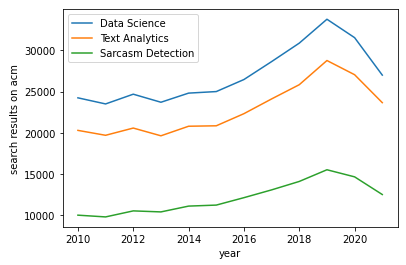
\includegraphics[width=0.45\textwidth]{./sources/search_results}
    \caption{Search results on the ACM Digital Library per Keyword}
    \label{fig:search_results}
\end{figure}

Collecting and analysing data from microblogging websites, like Twitter, Instagram or Facebook, quickly brings up the problem how to extract useful information from text. The field of natural language processing offers numerous different ideas and algorithms for all kind of textual challenges. Language detection, argument extraction or sentiment analysis are among the most popular tasks here. Especially in sentiment analysis, where the goal is to find out if the text tends to be positive or negative, sarcasm and irony can have a strong influence on the results.  

Of course sarcasm and irony do appear in many different kinds of text. But in scientific papers, structured documents or news articles those are way less used. Because of that research typically focuses on microblogging.

In fact the most common real-world use case for sarcasm detection is sentiment analysis. Companies want to extract the sentiment of user-comments to analyse how people react to their content. As an example take the user-comment "Best Smartphone ever!", that could be posted under an Amazon page showing a new smartphone. The first association of most people probably would be that the mentioned smartphone is actually good. So would the most sentiment analysis algorithms. Now imagine the same comment as some kind of review for the smartphone next to a bad rating (1 out of 5 stars in the Amazon example). Probably most people would change their opinion about the smartphone and think of the comment as sarcastic. For text analytics algorithms it's rather difficult to detect such kind of subtle hints.

Nevertheless many scientific works provide ideas how to deal with sarcasm and irony detection. In this work the current research state is summarized to give an overlook about the field, it's problems and the ways to deal with them. In detail the following questions are discussed:
\begin{enumerate} 
	\item What are the main problems when detecting sarcasm or irony in texts?
	\item Which groups of methods can be identified from previous works?
	\item What are good baseline algorithms for sarcasm detection? And how do more complex models perform in comparison to those baselines?
\end{enumerate}


The next section will point out how sarcasm and irony are defined, and what the differences between those are. Following that section three explains the problems with detection and why it's especially difficult in this field of text analytics. In section four different methods for sarcasm detection are explained and the methods are grouped in respect to the key ideas behind them. After that the explained methods are compared in section five and the pros and cons are discussed in section six. To finalize this work in the last section a conclusion is provided, summing up the main points and showing some ideas for future research.



\section{Language theory}
\label{lang-theo}

When trying to detect irony and sarcasm we first have to understand the differences between those two terms. The Cambridge Dictionary dictionary \footnote{https://dictionary.cambridge.org/} defines sarcasm as "the use of remarks that clearly mean the opposite of what they say, made in order to hurt someone's feelings or to criticize something in a humorous way". In the Oxford Learners Dictionary \footnote{https://www.oxfordlearnersdictionaries.com/} a similar definition goes "a way of using words that are the opposite of what you mean in order to be unpleasant to somebody or to make fun of them". From that can be seen, that sarcasm has to main concepts 1) it expresses the opposite of what is written and 2) it's used to mock or make fun of someone.

Coming to irony the definitions are very similar. Again the Cambridge Dictionary says "[irony is] a situation in which something which was intended to have a particular result has the opposite or a very different result". The Merriam-Webster Dictionary \footnote{https://www.merriam-webster.com/} defines irony as "a situation that is strange or funny because things happen in a way that seems to be the opposite of what you expected", but also as "the use of words that mean the opposite of what you really think especially in order to be funny". So irony is a concept that again 1) intends to express the opposite of what is said or going to happen and 2) mostly relates to situations.

Solely from the given definitions it's hard to draw a clear line between irony and sarcasm. And the science world aswell seems to be doubtful over the exact differentiation. Many studies treat them as very closely related concepts. So does S. Attadore \cite{Irony-as-relevant-inappropriateness} who claims that "Sarcasm is an overly aggressive type of irony". R. Gibbs and J. O'Brien \cite{Psychological_aspects_of_irony_understanding} go even further than that and do not substantially differentiate between sarcasm and irony in their work. Other authors try to make a clear distinction between the two concepts. J. Haiman \cite{Sarcasm-as-theater} believes that it is important to treat irony and sarcasm as different concepts. This opinion is also shared by Schaffer \cite{Vocal-Cues-for-Irony-in-English} and by D.Sperber and D. Wilson \cite{Irony-and-the-use-mention-distinction}.

In their work "An Empirical, Quantitative Analysis of the Differences Between Sarcasm and Irony" J. Ling and R. Klinger \cite{diff_irony_sarcasm}, criticize that most predictive models treat sarcastic and ironic tweets as the same. However their work shows, that it's actually a harder task to differentiate between sarcastic and irony tweets, than to treat them as a the same and try to detect them out of regular tweets. So this perhaps hints that it would be useful for modern models to not separate, between sarcasm and irony but rather treat them as the same. 

For reasons of simplicity in this work irony and sarcasm will be treated as the same concept. So when talking about sarcasm detection or irony detection the same idea of detecting sarcasm and irony out of literal text is meant.

When comprehending sarcasm humans often take situational context or details they know about the topic into account. In example if humans know each other very well, they'll have background information that makes it easier to figure out if a sentence was meant sarcastic or not. Regularly a special gesture or emphasis can hint sarcastic meanings. In text those subtle hints are missing. If people know each other well, the understanding of sarcasm still works fine. For other cases people came up with subtle hints for text, like special emojis or the use of \#irony and \#sarcasm on twitter.  A newer trend on the forum-like platform Reddit, where users hardly know anything about the other person posting, is marking ones posts with '/s' (short for /sarcasm). 


\section{Problems in sarcasm detection}

When transferring the problem of understanding sarcasm from humans to computers, those subtle hints among many other factors raise problems that haven't been completely overcome in research yet. 

% Context Information
Perceiving context information is a task, that humans perform subconscious. But for computers that's anything else but trivial. Previous work \cite{The-Role-of-Conversation-Context-for-Sarcasm-Detection-in-Online-Interactions} has shown that models with any kind of contextual understanding do outperform models without context knowledge. In the work " Twitter Sarcasm Detection Exploiting a Context-Based Model" by Z. Wang et al. \cite{Twitter-Sarcasm-Detection-Exploiting-a-Context-Based-Model}, the researchers explored that thought of generating context even further. They introduced three different ways of context generation. First taking preceding and follow-up tweets from the same author into account to generate history-based context. Secondly only using preceding tweets but from other authors aswell to generate how they call it conversation-based context. And lastly only looking at preceding tweets with the same hashtag for so called topic-based context.
By testing different ideas of how context can be embedded in sarcasm detection, they found out that context information can improve the performance of models. Further they also showed that it's important to carefully choose how context information can be fed into a detection model. If done wrong providing any contextual information can be harmful and significantly lower the performance results.
Also when working with any kind of contextual information overfitting-like problems can occur. Training an model on a specific type of context can indeed increase it's performance, but also lowers it's generalization ability. Therefor the model then performs worse when confronted with slightly different tasks (i.e. conversing from detecting sarcastic tweets to sarcastic facebook comments). Whereas models without context information mostly have a better generalization.

% microblogging data
Another problem that's indirect connected to sarcasm and irony detection is the hard to work with data. In text analytics working with microblogging-datasets like tweets or user comments is generally known as hard to work with data. As already explained this type of data is still preferred when researching sarcasm or irony detection because those concepts are just more frequently used here than for example in news articles or official documents. The details about why it is so hard to work with mircoblogging-datasets and what could be good preprocessing steps have been looked into by many other authors \cite{The-effect-of-preprocessing-techniques-on-Twitter-sentiment-analysis} \cite{Analysis-of-Twitter-Specific-Preprocessing-Technique-for-Tweets} \cite{Effective-Text-Data-Preprocessing-Technique-for-Sentiment-Analysis-in-Social-Media-Data} \cite{Efficient-Algorithms-for-Preprocessing-and-Stemming-of-Tweets-in-a-Sentiment-Analysis-System} already. Since this is a broad research field by itself it won't be covered in more detail in this work.

% To-Do:Wrong annotations (hashtags vs. humans)
% imbalanced data
When creating a own dataset for sarcasm detection, researchers often come across the problem of imbalanced data. A balanced dataset would consist of 50\% sarcastic and 50\% non-sarcastic tweets. For an unbalanced dataset this distribution would shift. When collecting data from twitter the dataset normally consist of only a small percentage of sarcastic tweets. To still have enough sarcastic tweets to effectively train a model the dataset would need to be very large. Researchers often avoid this by choosing an even amount of sarcastic and non-sarcastic tweets for their dataset.


%growing language / fast-paced changes
In a work from 2021 T. Jain et al. wrote "Another major challenge is the growing size of the languages. Every day hundreds of new slang words are being created and used on these sites" \cite{Sarcasm_detection_of_tweets}. Models that are trained on datasets could quickly struggle when faced with those fast paced change of languages. Therefor, instead of scraping datasets from the real world, they introduced a seeding algorithm which generates random training sets. This helped the model to keep foot with the never-resting language growth.
Also most language processing are working with an bag-of-words implementation. Here the frequency of occurences of words is used as a feature. Rather newly invented slang words can have unwanted impacts because they are likely to be especially rare in a text context.

% idiomatic expressions
One problem that is overlooked or just taken as granted in most works is that sarcasm sometimes can be hidden in slight changes. A. Joshi et al. \cite{Automatic_Sarcasm_Detection} provide a good example for this problem: The sentence "I love it when my son rolls his eyes on me" clearly is sarcastic and means the opposite of what is written. But the very similar sentence: "I love it when my son gives me a present" is non-sarcastic. Humans are trained with this kind of idiomatic expressions, and automatically connote rolling eyes as negative. Different cultures or social groups may have different expressions or gestures but most are broadly understand (another example could be pointing up the middle finger). Computers miss this understanding.

Further much literature does not differ between sarcasm/irony and hidden bragging. An example of hidden bragging is "I failed this test so hard. Only got 95 out of 100 points." and as the name says it's mostly used to hide the intent of bragging behind an innocent statement. To our best knowledge there isn't much work that looks into how this concept differs from sarcasm and if marking it could improve sentiment analysis.



\section{Methods for sarcasm detection}

In this section different types of methods that have been published in literature so far are listed. The general idea behind the method groups are explained and one or two selected works applying this technique are explained in more detail. The comparison and discussion of those methods is done in the following sections.
All of the methods listed are trying to solve the classification problem if a text is sarcastic or non-sarcastic. The data used by the methods are mostly tweets.

\subsection{Baseline methods}

Providing comparable baselines for sarcasm detection is not trivial, since most works choose their own baselines and to our best knowledge no gold-standard for benchmarking is existent. Therefor the baseline methods in this work are chosen by two criteria. First criterion is if the method is a more simple attempt and avoids training complex models. Secondly the work has to be stable and believed to perform well over a broad variety of datasets instead of being focused on specific data. 
In the Following selected works that fulfill these criteria are explained and serve as a baseline to compare the more complex methods to later on.

The first baseline method was published by A. Reyes et al. in 2013 \cite{A-multidimensional-approach-for-detecting-irony-in-Twitter}. In their work they detect different features from short texts using lexical theories. As data they used tweets that have been tagged with \#irony or an thematic hashtag like \#politics. Overall they worked with 40.000 tweets, divided into four different sets. Out of this tweets the authors extracted different linguistic features with which they later trained their models.
As algorithms two algorithms, that are very common in literature, have been used: 'Naive Bayes' and 'Decision Tree'. To truly evaluate their performances they tested their model using first an balanced dataset (50\% sarcastic tweets, 50\% non-sarcastic tweets) and later an imbalanced dataset (30\% sarcastic tweets, 70\% non-sarcastic tweets). The models achieves performances up too 78\% precision and 74\% recall. The Decision tree method overall performs slightly better than Naive Bayes. In general the prediction is significantly better on balanced than on imbalanced sets.

Another noteworthy baseline was published by P. Carvalho at al. aready in 2009 \cite{Clues-for-Detecting-Irony-in-User-Generated-Contents}. Remarkable in this work is, that the authors didn't work with tweets or social media data (probably because twitter had been founded only three years before this work had been published). Instead they tried to detect irony and sarcasm in user-comments submitted to an online-newspaper. 
Compared to nowadays more complex models they attempted a rather simple approach. To distinguish sarcastic and normal comments they identified four markers for sarcastic comments: 1) emoticons and written examples for laughing (i.e. "lol" or "haha"), 2) heavy punctuation marks, 3) quotation marks and 4) positive interjections.
Their works shows that these sarcastic patterns are present significantly more often in sarcastic than in non-sarcastic comments. Applying all those patterns they reach a mean precision up too 61,07\%.


\subsection{Pattern-based methods}

Pattern based approaches for sarcasm detection are based on the key idea, that sarcastic or ironic sentences follow special language patterns. They often use Part-of-Speech-Tagging (POS-Tagging), a technique that transform sentences into a list where every word is assigned it's part of speech. For the tagging often language dependent corpora like the Brown corpus \footnote{Brown Corpus: http://korpus.uib.no/icame/manuals/BROWN/INDEX.HTM} for english language are used. An example how POS-tagging works can be seen in Table \ref{tab:pos}. The exact tagging may vary between different implementation but the key idea stays the same.
\begin{table}[h]
\begin{tabular}{|c|c|c|}
\hline
\textbf{sentence} & \textbf{part of speech}                                     & \textbf{pos-tag}                                \\ \hline
The               & article                                                     & AT                                              \\ \hline
quick             & \begin{tabular}[c]{@{}c@{}}adjective \\ adverb\end{tabular} & \begin{tabular}[c]{@{}c@{}}JJ\\ RB\end{tabular} \\ \hline
brown             & \begin{tabular}[c]{@{}c@{}}adjective\\ adverb\end{tabular}  & \begin{tabular}[c]{@{}c@{}}JJ\\ RB\end{tabular} \\ \hline
fox               & noun                                                        & NN                                              \\ \hline
\end{tabular}
\caption{Example for POS-Tagging}
\label{tab:pos}
\end{table}

Commonly datasets from twitter are used and annotated whether a document is sarcastic or non-sarcastic. Once those used documents are tagged a range of algorithms can be used to detect pattern. Often used for this are algorithms like Support Vector Machines (SVM) or k-Nearest Neighbours (k-NN). After the sarcasm-patterns are calculated the algorithms are applied on testing data to check the performance of the patterns.

In their work "A Pattern-Based Approach for Sarcasm Detection on Twitter" \cite{pattern} M. Bouazizi and T. Ohtsuki implemented such a pattern-based technique. They also used twitter data to extract and test the patterns. The patterns were grouped into 4 main groups:
\begin{itemize}
 \item Sentiment-Related Features: words (especially adjectives) are marked whether they are positive (i.e. "happy", "like") or negative (i.e. "sad", "angry"). If a sentence contains positive and negative marked words a sarcastic-pattern is retrieved.
 \item Punctuation-Related Features: They claim special punctuation, like many exclamation marks, many question marks, over extensive use of vowels and so on indicate sarcastic meaning.
 \item Syntactic and Semantic Features: Common expressions or the use of uncommon words are identified as sarcastic patterns. As an example "... love NOUN when ..." hints the sarcasm in the sentence "I love it when I have to stand up early".
 \item Pattern-Related Features: Here patterns that are not present in the previous features, but still can be extracted from the used data are grouped. A pattern here consists of a fixed order of POS-tags with a special length that appears at least 2 times in the used data. Also patterns that appear in sarcastic as well as non-sarcastic tweets are filtered out because they're not correlated with sarcasm.
\end{itemize}

M. Bouazizi et al. then ran classification with those patterns using Random Forest, SVM, k-NN and Maximum Entropy. They measured their performance using Accuracy, Precision, Recall and F1-Measure. The results showed they significantly outperformed given baselines. Detailed results can been seen in Table \ref{tab:perf}, and are compared to the other methods in a later section.


\subsection{Rule-based methods}

The key concept behind rule-based approaches is to detect sarcastic tweets based on specific markers. Those markers are detected using rules that the researchers defined beforehand. A simple example for such a rule could be: "If a tweet contains \#sarcasm it is more likely to be sarcastic". Rule-based approaches are similar to pattern-based ones. However the difference is that rule-based methods are more focused on semantic features or more general patterns in the text, whereas the pattern-based approaches are trying to detect detailed syntactic word patterns. Also rules get defined by researchers beforehand, whereas patterns can also be detect in given data.

On social media data hashtags can be a strong cue for the sentiment of the tweet. D. Maynard et al. \cite{Who-cares-about-sarcastic-tweets?} tried to prove this hypothesis by extracting a tweets sentiment based on a corpus of rules. A tokeniser was used that identifies hashtags and splits combined hashtags into single words (as example \#conflictpalmoil was tokenised as 'conflict', 'palm' and 'oil'). Now their rules were applied on the split hashtags to identified the tweets sentiment. Chosen examples of those rules and how they predict sentiment are shown in Table \ref{tab:rules}. Notice how especially the second tweet which contains 'best feeling in the world' as a strong positive marker still gets a negative sentiment.

\begin{table*}[t]
\begin{tabular}{ccc}
\textbf{rule}                                                                                                                                                                  & \textbf{tweet}                                                                                                   & \textbf{final sentiment} \\ \hline
\begin{tabular}[c]{@{}c@{}}If there is a single hastag denoting sarcasm,\\ and the original sentiment is positive or neutral,\\ we flip the polarity to negative.\end{tabular} & \begin{tabular}[c]{@{}c@{}}It's not like I wanted to eat breakfast anyway. \\ \#sarcasm\end{tabular}             & negative                 \\ \hline
\begin{tabular}[c]{@{}c@{}}If there is more than one hashtag,\\ we look at any sentiment contained in those hashtags.\end{tabular}                                              & \begin{tabular}[c]{@{}c@{}}The best feeling in the world is being ignored. \\ \#bestthingever \#not\end{tabular} & negative                 \\ \hline
\begin{tabular}[c]{@{}c@{}}If two hashtags both contain sarcasm indicators,\\ we treat them as one single sarcasm indicator.\end{tabular}                                      & \begin{tabular}[c]{@{}c@{}}You are really mature. \\ \#lying \#sarcasm\end{tabular}                              & negative                 \\ \hline
\end{tabular}
\caption{Examples for rules to detect sentiment using hashtags (based on \cite{Who-cares-about-sarcastic-tweets?})}
\label{tab:rules}
\end{table*}

M. Abulaish et al. \cite{Self-Deprecating-Sarcasm-Detection} published a work that investigates a more niche topic of sarcasm detection namely self-deprecating sarcasm. This special kind of sarcasm mostly is used by users to joke about themselves. They implemented an algorithm to detect tweets that are self-centered. For this the algorithm included special filter rules that were applied on pos-tagged tweets. Afterwards they checked the filtered tweets whether or not those were sarcastic. Overall they reported strong results on balanced as well as imbalanced datasets.  

\subsection{Learning-based methods (Statistic-based methods}

In literature learning-based methods are also referred to as statistical methods. This is because the algorithms used in this group are based on statistics and are commonly used in the field of machine learning. Typical examples are Naive Bayes, Support Vector Machines (SVM) or simple distance based metrics. When training these statistical models features have to be derived from the data and given to the algorithm. The works published in the field of sarcasm detection using learning-based methods differ in terms of features they used and algorithms chosen.

A method that is based on distance metrics was published by O. Tsur et al. in 2010 \cite{ICWSM}. They attempted to recognize sarcasm in Amazon product reviews. As features they combined syntactic evidence based on punctuation and spelling with pattern-based features where they looked at the text content. For the classification they created feature vectors for each sample in the test- and training data. By computing euclidean distances the k-nearest neighbours had been found. Between those a weighted mean was computed to label the current sample with a score between 1 (not sarcastic) and 5 (definitive sarcastic). The method of 5-fold cross validation was used to evaluate the performance of their method reporting good results (see Table \ref{tab:perf}).

Another work from D. Ghosh et al. published in 2015 \cite{Sarcastic-or-Not} re-defines the sarcasm detection problem as a word sense problem. Claiming if a word has literal sense it's non-sarcastic whereas if a words sense isn't literal it's sarcastic. They also worked with tweet data that had been labeled by the hashtags included in the tweets. Tweets with \#sarcasm are labeled as sarcastic meanings whereas tweets with hashtags like \#happy are labelled as literal meaning. From these tweets the authors extracted target words that can been as features for sarcastic or literal meaning. To classify a tweet distributional methods have been compared with support vector machines containing different kernels. The best results have been reported using SVM. 


\subsection{Deep learning methods}

The vast majority of what is commonly seen as state-of-the-art methods can be found in this subsection. The usage of deep learning methods like neural networks is not new to computer scientists, but had a strong rise in popularity over the last years.
To effectively use a deep learning technique in general three things are necessary. Firstly a big amount of data to train and evaluate the models is needed. A clear statement about what is enough data cannot be made, but having more data available usually doesn't hurt the research.
Next to data a good deep learning technique is needed. There exist thousands of different models and architectures published in previous works. Finding or building a good one is a challenging task. Often researchers also simply make some adjustments to existent models to improve performance by a few percentage points. In their book "Deep Learning" I. Goodfellow, Y. Bengio and A. Courville \cite{goodfellow2016deep} describe the neural network cosmos in detail. 
The last thing needed to work effectively with deep learning methods is computing power. Neural networks frequently perform a lot of calculations. To train and evaluate models in an acceptable period of time a lot of computational resources are needed.

When transferring these concepts over to nlp-problems and especially sarcasm detection the data mostly comes from tweets or social media due to previous described reasons. Nowadays most researchers also have access to performant computing clusters. The only thing left is choosing a good deep learning model. Those range from more simple feed-forward architecture, over recurrent neuronal networks (RNN) up to highly complex BERT-architectures \footnote{Bidirectional Encoder Representations from Transformers: a state-of-the-art language model first published by Google in 2018}.

In 2016 S. Amir et al. \cite{Modelling-Context-with-User-Embeddings-for-Sarcasm-Detection-in-Social-Media} published a deep learning method for sarcasm detection based on a convolutional neural network (CNN). Their model combines user embeddings with features that are extracted from the text. User embeddings project similar users closely together. This is done because the authors follow the hypothesis that "[user embeddings] will naturally capture some of the signals that have been described in the literature as important indicators of sarcasm". Those embeddings are contextual informations, allowing the model to take into account who authored a tweet and based on that change the probability of it being sarcastic. Indeed the authors showed that those user embeddings improve the performance of the model by a few percentages. 
The main part of the model still used features that are extracted from the input texts. The features are extracted using word embeddings, a common nlp-technique that maps words into vectors. This has the advantage that features don't have to be designed manually but instead are learned by the model from the given input data. When comparing their model with another one that needs this manually feature extraction the authors reported a slight increase of performance as well as stability. S. Amir et al. reported the best results when they combined those feature vectors with the information gained from the user embeddings.

When talking about deep learning and natural language processing a model architecture called 'Transformers' can't be left unmentioned. Original introduced in 2017 by a team of Google Researchers \cite{transformers} the architecture combines many machine learning best-practice methods (like en- and decoders) into an efficient model. Based on the ideas behind transformer architecture another team from Google AI Language created the Bidirectional Encoder Representations from Transformers widely known as BERT \cite{BERT}. This model uses especially the encoder part from the typical transformer architecture and is specialized for text analytics tasks. Due to it's high complexity training a BERT model form scratch takes a lot of time. However a big advantage of the architecture is that a pre-trained model only needs some time efficient fine-tuning and it can be used for many different nlp-tasks like question answering or language inference. Because of this highly flexible architecture a whole family of BERT-like models have been published in the last years. Some of them only containing changed input/output layers while others added some additional layers or introduced some other changes. The scientific world also became creative with naming and models like RoBERTa, AlBERTo or BERTje have been published.

Based on the BERT architecture R. Potamias et al. in 2020 \cite{A-Transformer-based-approach-to-Irony-and-Sarcasm-detection} published a model that uses this technique to detect irony and sarcasm. In fact they build a recurrent CNN based on the RoBERTa model (RCNN-RoBERTa). The pre-trained RoBERTa model is used to map words into an lower dimensional embedding space. This output is then fed into the recurrent and convolutional layers, which are there to capture sequential relationsships between the words. Again this model isn't dependent on manually extracted features but instead learns important features on it's own from the training data. The authors claim that this in addition with some other preprocessing steps like stemming that can be left out with RCNN-RoBERTa reduce the computation costs significantly.


\subsection{Out-of-the-box methods}

In this section some methods that don't follow the usual approaches or have a slightly different use-cases are listed. They do not fit in any of the previous groups but still are valuable research and maybe motivate that it can be worth thinking outside the box sometimes.

Many of the previous layed out works extract feature vectors from the input texts. Some even enrich them with additional information in example author names. A. Mishra et al. \cite{eye-patterns} proposed a method that additionally enriches feature vectors with eye patterns of humans reading a text. They claim that eye-patterns when reading sarcastic texts differ from those of normal texts. 

\begin{figure}[H]
    \centering
    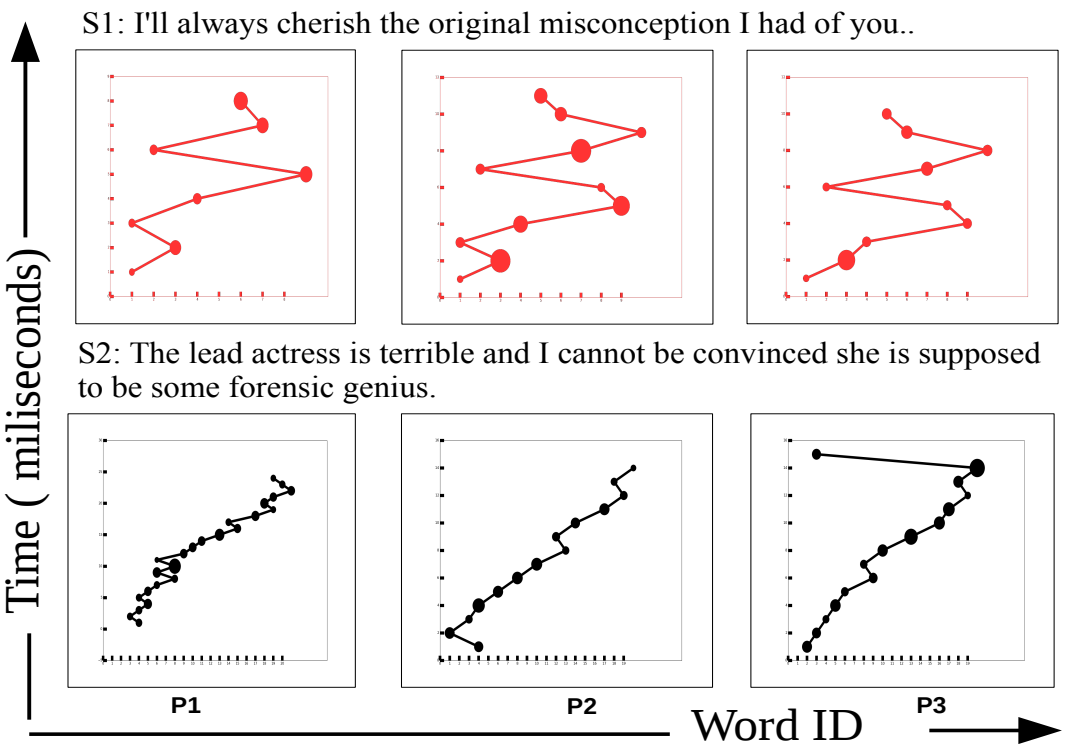
\includegraphics[width=0.45\textwidth]{./sources/eye_patterns}
    \caption{Eye-Patterns of persons reading sarcastic (S1) and non-sarcastic (S2) sentences \cite{eye-patterns}}
    \label{fig:eye_patterns}
\end{figure}

Figure \ref{fig:eye_patterns} shows three participants from their study reading a sarcastic sentence (S1) and a non-sarcastic sentence (S2). From the eye-movements the order in which the words were read have been plotted in each box. When reading the sarcastic sentence the reading-pattern is more zig-zag and erratic. The non-sarcastic sentence shows a mostly clear and linear pattern. In their work they showed how to extract those patterns and use them as additional information. Using already existent models and data they have been able to improve performances by some percentage points. 


\section{Comparison}

%%%%%%%%%
\begin{table*}[t]
\begin{tabular}{|c|c|c|c|c|c|c|}
\hline
                                                                                           & \textbf{}                                                                           & \textbf{Accuracy} & \textbf{Precision} & \textbf{Recall} & \textbf{F1-Measure} & \textbf{Data}                                                                                   \\ \hline
\multirow{2}{*}{\textbf{\begin{tabular}[c]{@{}c@{}}baseline\\ methods\end{tabular}}}       & \cite{A-multidimensional-approach-for-detecting-irony-in-Twitter}                   & -                 & 0,780              & 0,740           & 0,760               & Tweets (annotated by hashtags)                                                                                         \\ \cline{2-7} 
                                                                                           & \cite{Clues-for-Detecting-Irony-in-User-Generated-Contents}                         & -                 & 0,611              & -               & -                   & user-comments in online-newspapers                                                              \\ \hline
\textbf{\begin{tabular}[c]{@{}c@{}}pattern-based\\ methods\end{tabular}}                   & \cite{pattern}                                                                      & 0,831             & 0,911              & 0,734           & 0,811               & Tweets (annotated by hashtags)                                                                   \\ \hline
\multirow{2}{*}{\textbf{\begin{tabular}[c]{@{}c@{}}rule-based\\ methods\end{tabular}}}     & \cite{Who-cares-about-sarcastic-tweets?}                                            & -                 & 0,910              & 0,910           & 0,910               & Tweets (annotated manually)                                                                      \\ \cline{2-7} 
                                                                                           & \cite{Self-Deprecating-Sarcasm-Detection}                                           & -                 & 0,970              & 0,920           & 0,950               & Tweets (annotated manually)                                                                     \\ \hline
\multirow{2}{*}{\textbf{\begin{tabular}[c]{@{}c@{}}learning-based\\ methods\end{tabular}}} & \cite{ICWSM}                                                                        & -                 & 0,766              & 0,813           & 0,788               & \begin{tabular}[c]{@{}c@{}}Amazon Reviews \\ (semi-supervised, annotated manually)\end{tabular} \\ \cline{2-7} 
                                                                                           & \cite{Sarcastic-or-Not}                                                             & -                 & 0,870              & 0,856           & 0,863               & Tweets (annotated by hashtags)                                                                  \\ \hline
\multirow{2}{*}{\textbf{deep learning methods}}                                            & \cite{Modelling-Context-with-User-Embeddings-for-Sarcasm-Detection-in-Social-Media} & 0,872             & -                  & -               & -                   & Tweets (pre-existent datasets)                                                                  \\ \cline{2-7} 
                                                                                           & \cite{A-Transformer-based-approach-to-Irony-and-Sarcasm-detection}                  & 0,910             & 0,900              & 0,900           & 0,900               & 4 pre-existent datasets                                                                         \\ \hline
\begin{tabular}[c]{@{}c@{}}\textbf{out-of-the-box methods}\end{tabular}  & \cite{eye-patterns}                                                                      & -    & 0,765     & 0,753  & 0,757      & short-texts (own dataset)                                                                   \\ \hline
\end{tabular}
\caption{Reported performances of previous explained methods}
\label{tab:perf}
\end{table*}
%%%%%%%%%% 

In this section the previously explained methods are objectively compared. For an detailed discussion over the pros and cons have a look at the following section. Table \ref{tab:perf} contains the reported performances of the papers explained beforehand. Note that only the best result that each work reached is shown. Although most of the works are based on twitter data, they still have different datasets to train and test their performance. Therefor a direct comparison of the values cannot be made due to this differences in used data. However this section is comparing the reported works with focus on other aspects.
All performances are listed (as longs as provided by the authors) with four different measures namely Accuracy, Precision, Recall and F-Measure.

\begin{itemize} 
	\item Accuracy: it's a measure to represent the overall correctness of the model. It calculates the fraction between all correct classified instances divided by the number of all instances.
	\item Precision: it's calculated by the fraction of instances that successfully have been classified as class x (true positives) divided by the sum of all instances that have been classified as x (true positives + false positives).
	\item Recall: it's calculated by the fraction of instances that successfully have been classified as class x (true positives) divided by the sum of instances that actually are class x in the ground truth (true positives + false negatives).
	\item F1-Score: the F-Score combines precision and recall into one measure moving between 0 and 1. The F1-Score is calculated multiplying 2 with the product of precision and recall divided by the sum of precision and recall. It's also known as the harmonic mean between precision and recall.
\end{itemize}

Most of the publications listed in Table \ref{tab:perf} reported their precision and recall values. Commonly achieving good results with their proposed methods on their own data. Only a few of them have chosen to also check the performance of their methods on other datasets. A commonly used benchmark dataset for sarcasm detection is not existing to this point, what again makes a comparison of achieved results between different methods complicated.

Also it can be seen that most of the works use data from Twitter for training and evaluating their models. However the technique used for annotating the data varies between manually labeling and annotations by hashtags. When manually labeling data the researchers themselves or other people read the texts and decide whether or not the text is sarcastic. When annotations are done via hashtags the content of the tweet is decisive about it's class. Typically if a tweet is tagged with \#sarcasm or \#irony it gets counted as saracstic. For non-sarcsastic tweets the absence of \#sarcasm could be an indicator but mostly is not enough. Therefor often other hashtags like \#politics or \#happy are used, because they are thought of including very less sarcasm.
 
Another point the methods differ in is the set of features chosen and the feature extraction methods. Depending on the methods the features are either defined by the researchers, like in rule-based or statistic-based methods. Here often semantic, contextual or syntactic features are chosen. Whereas in deep learning methods or pattern-based approaches the features are more commonly detect by the used algorithms based on the training data. Features are more likely to represent the actual content represented in the input texts.

\section{Discussion}

This section provides a discussion about different techniques and their respective advantages or disadvantages. First of all the established practice of using Twitter data has some major advantages. Social media data is known to be quite challenging in the field of text analytics, due to it's unclear structures and no rules it follows. Still training a model with such relatively hard data makes it more robust against more easy data. Also because the data being so diverse many edge-cases already are inherent and tested during the research.

Nevertheless data annotation is a challenging problem in sarcasm detection. In the language theory section it is argued that no clear definition for the concepts of irony and sarcasm can be given. Further we humans don't share a mutual understanding what is sarcastic and what not. This makes human based annotations difficult and error prone, the interrater agreement becomes low. Also having humans actually read and label data normally is very costly and time-consuming. 
On the other hand hashtag-based annotations only shift this problem. Again humans, this time the authors of the respective tweet, are classifying if their tweet is sarcastic or not. Again the missing collective understanding of sarcasm and irony is problematic. There is no control how authors tag their tweets, so they could use \#sarcasm in a tweet that other humans wouldn't classify as sarcastic. But at least this time the tweet authors can decided whether or not their tweet is meant sarcastic. Also hashtag-based annotations are more cost- and time-efficient.

When using hashtag-based labelling it also needs to be discussed how to choose non-sarcastic tweets. The absence of a hashtag that marks sarcasm or irony is very important here. But it is not reliable enough to classify a tweet as non-sarcastic. Many works therefor also used hashtags like \#politics or \#happy. Especially \#politics is seen as not including much sarcasm. Those in general are efficient markers. However when using those there could be a bias included. In example when only using \#politics as marker for non-sarcastic tweets, a model could be accidentally trained to detect politic tweets out of others instead of detecting sarcasm. For this reason we suggest using multiple different hashtags, from different topics, as markers for non-sarcastic tweets.

Further the features used to identify sarcasm or irony and methods used for extraction need to be discussed. When the researchers decide about what are important features they have more control over the model and what gets detected or not. Also it can be determined what features influenced the resulting class of a sample. A disadvantage here is that unknown or unnoticed characteristics of sarcasm can't be detected what may impair the overall performance.
When using in example neural networks to classify sarcasm, often it can't be clearly told what factors lead to an specific output. The model is a sort of black box that generates an output to any given input. Because such algorithms can extract important features on their own from the training data it is possible to detect features researchers haven't thought about or are unaware of. This can lead to increased performance, but fine-tuning these models to detect the wanted features can be rather difficult.

An additional piece of information, for which it is unclear how important it is, is the text-context. Some works tried to enrich their model-inputs with context information, in example tweet histories or author information. Mostly reporting a little improvement in performance measures. But context information is not always at hand or easy to obtain. Also models need to be modified to effectively handle context information, what can be a big effort. If it's worth and useful to work with context information depends on the given task and many works also reported good results without it.


\section{Excourse: Other Languages and sarcasm}

The whole research layed out so far focused on sarcasm detection in the english language. Since english is the most common language in the world it's sort of a best practice for publications to focus on it. Nevertheless there exist a few publications that looked at the problem in different languages. Next to english there are a lot of papers existent that look at sarcasm detection in the chinese language. Also for languages like spanish and portugese there have been some papers published. This isn't surprising since those are among the most spread languages in the world.

But also a few not that common languages have interesting works published about. In example T. Ptácek et al. worked on a baseline and a dataset for sarcasm detection in czech \cite{czech}. Although their reported results were a lot lower than their english comparison it's still a promising baseline for future works. In 2014 D. Al-Ghadhban and his colleagues published a work that classifies arabic tweets whether they are sarcastic or not \cite{arabic}. They reported measure of recall, precision and f-measure of 0.659, 0.710 and 0.676. Another language that has been covered by researchers is dutch. C. Liebrecht et al. \cite{dutch} trained a machine learning classifier with about 78 thousand dutch tweets. Furthermore Vries et al. developed BERTje \cite{bertje}, a BERT-architecture for the dutch language, that outperforms multilingual BERT models.

There exist very less comparable research in other languages than english what makes it difficult for researchers to set their foot in those areas. Also the change of language can challenge modern state-of-the-art algorithms. But we believe the most challenging point for sarcasm detection in other languages is the change of culture. In different regions the way how sarcasm or irony is used varies. That not only changes syntatic patterns but also semantic features. So sarcasm detection in other languages is a difficult yet exciting research field.


\section{Conclusion}

Humans don't seem to have the same clear understanding about what is sarcasm or irony. One indication for that is the scientific dispute about whether or not these ideas are the same or have different characteristics. Another supporting argument for this is the fact that humans themselves are struggling with labelling sarcastic and non-sarcastic sentences. This shows that there is no definite understanding what sarcasm is but rather an unclear perspective that slightly differs between all individuals.

In this work an overview of the research field irony and sarcasm detection was given. It was shown how different previous works approached the problem and came up with different ideas. The most common problems when working in sarcasm detection had been pointed out. To quickly recap those were the inherent problems when working with microblogging or social media data, their difficult preprocessing and fast-paced language changes. Also the important role of context and how it can be used in sarcasm-detection models was explained. 

Those problems made it clear why this task is so challenging for computers. Nevertheless there exist many attempts to deal with this problem. We grouped the attempts into six different categories. For each category selected publications and models were explained.

More simple rule-, pattern- or statistic-based methods achieved good results. However when looking at more recent publications a clear trend towards the more machine learning based or even deep learning techniques can be detected. The newest research in this field shows promising deep learning models and even uses a variety of BERT-architectures to classify sarcasm. 

The explained methods were compared, listing their reported performances and data they used. A direct comparison of the performances was difficult, because of problems like data variety and missing benchmarks. Still some more general points like chosen data or feature extraction had been compared. Following this comparison we also provided a discussion of the mentioned points. Also picking up some of the problems named earlier and discussing ways to solve them. We pointed out some of the advantages and disadvantages of one or the other way.

The field or sarcasm detection is currently a highly researched topic in text analytics with lots of papers published in the last couple years. However there are still some points that haven't been looked at or need some further research. As discussed the most work focuses on the english language, what is a good best practice for research, but other languages are mostly unexplored. Further the dominant data type is social media. Little to less works looked at other data like newspapers, blog articles or even political speeches. Such research may change the problem away from detecting sarcasm for sentiment analysis to maybe detecting sarcasm for the problem of argument extraction. As an example it could be interesting if and how politicians hide their arguments inside sarcastic phrases. 


%%
%% The next two lines define the bibliography style to be used, and
%% the bibliography file.
\bibliographystyle{ACM-Reference-Format}
\bibliography{sample-base}

%%
%% If your work has an appendix, this is the place to put it.
\appendix

\end{document}
\endinput
